\subsection{Elementare Funktionen (Teil 1)}
\subsubsection{Polynome}
\paragraph{Def. 1:} \parskp
$y=f(x)=a_n\; x^n+a_{n-1}\;x^{n-1}+...+a_2\; x^2+a_1\; x+a_0$ mit $(a_0, ..., a_n \in \mathbb{R}, x\in \mathbb{R})$ heißt ganze rationale Funktion oder \emph{Polynom} vom Grad $n$ (falls $a_n \not = 0$).\\
Zur Beschreibung der Funktionswerte zweckmäßig: HORNER-Schema\\
(vgl. Stellenwertsysteme  \ref{Stellenwertsysteme})\\
\begin{tabular}{r | c c c c c c}
 & $a_n$ & $a_{n-1}$ & $ a_{n-2}$ & ... & $a_1$ & $a_0$\\
$x_0$ &  & $b_{n-1}\cdot x_0$ & $b_{n-2}\cdot x_0$ & ... & $b_1 \cdot x_0$ & $b_0\cdot x_0$ \\
\hline
 & $\underbrace{\boxed{b_{n-1}}}_{=a_n}$ & $\boxed{b_{n-2}}$ & $\boxed{b_{n-3}}$ & ... & $\boxed{b_0}$ & $f(x_0)=r_0$\\
\end{tabular}\\
Polynomdivision: $\frac{f(x)}{x-x_0}=b_{n-1}\;x^{n-1}+b_{n-2}\;x^{n-2}+...+b_1\; x + b_0 + \frac{r_0}{x-x_0}$

\subparagraph{Bsp. 1:} \parskp
$f(x)=x^5-2x^3+x^2-6$, \quad $x_0=3$, \quad ges: $f(x_0)$, \quad$\frac{f(x)}{x-x_0}$\\
\begin{tabular}{r| c c c c c c}
 & $1$ & $0$ & $-2$ & $1$ & $0$ & $-6$\\
$x_0=3$ &  & $3$ & $9$ & $21$ & $66$ & $198$ \\
\hline
 & $1$ & $3$ & $7$ & $22$ & $66$ & $192$\\
\end{tabular}\\
$f(x):(x-3)=x^4+3 x^3 + 7x^2+22x + 66 + \frac{192}{x-3}$

\paragraph{Satz 1:} \parskp
Es sei $f(x)=p_n(x) = a_n \; x^n + ... + a_0$ ein Polynom vom Grad $n$ (d.h. $a_n\not = 0$). Dann besitzt $f$ (in $\mathbb{C}$) genau $n$ Nullstellen $x_1,...,x_n$ und es gilt: $f(x) = a_n (x-x_1)\cdot (x-x_2)\cdot ... \cdot (x-x_n)$. (Zerlegung in Linearfaktoren)

\subparagraph{Diskussion:}
\begin{enumerate}
\item Falls in der Linearfaktorzerlegung der Faktor $(x-x_0)$ genau $k$-mal ($1\geq k \geq n$) vorkommt, so heißt $x_0$ \emph{$k$-fache Nullstelle} (Nullstelle der Vielfachheit $k$).
\item Nichtreelle Nullstellen sind möglich, sie treten stets paarweise als konjugiert komplexe Zahlen auf ($x_0, \overline{x_0})$). In diesem Falle Zusammenfassung der Linearfaktoren zu reellen quadratischen Faktoren möglich: $(x-x_0)\cdot (x-\overline{x_0})=x^2-(x_0 + \overline{x_0})x + x_0 \cdot \overline{x_0}=x^2-2\cdot Re(x_0) \cdot x + |x_0|^2$
\item Falls $a_0, a_1, ... , a_n$ ganze Zahlen sind, dann sind ganzzahlige Nullstellen Teiler von $a_0$ (falls vorhanden).
\item Allgemeine Methoden zur Nullstellenbestimmung später (Kap. 3 \ref{sec:3})
\end{enumerate}

\subparagraph{Bsp. 2:} \parskp
$p(x) = x^4 + x^3 -5x^2 + x-6$, \quad ges: Nullstellen\\
Durch Probieren $\boxed{x_1=2}$\\
mit HORNER-Schema:\\
\begin{tabular}{r | c c c c c l}
 & 1 & 1 & -5 & 1  & -6 & \\
$x_1=2$ & & 2 & 6 & 2 & 6 &\\
\hline
 & 1 & 3& 1 & 3 &$\boxed{0}$ & $\curvearrowright p(x) = (x-2)\cdot \underbrace{(x^3+3x^2+x+3)}_{\text{durch Probieren }x_2=-3}$\\
$x_2=-3$ & & -3 & 0 & -3 & & \\
\hline 
 & 1 & 0 & 1 &\boxed{0}& & $\curvearrowright p(x) = (x-2)(x+3)\underbrace{(x^2+1)}_{x_{3,4}=\pm i}$\\ 
\end{tabular}\\
$\curvearrowright$ Zerlegung: $p(x)= (x-2)(x+3)(x-i)(x+i)$

\subsubsection{Gebrochen rationale Funktionen}

\paragraph{Def. 2:} \parskp
$y=f(x) = \frac{p(x)}{q(x)}=\frac{a_m\; x^m + a_{m-1}\; x^{m-1}+...+a_1 \; x+a_0}{b_n \; x^n+b_{n-1}\; x^{n-1} + ... + b_1 \; x + b_0}$ mit $a_m \not = 0$, $b_n \not = 0$ und $ Db(f)=\{x\in \mathbb{R}| q(x)\not = 0\}$ heißt gebrochenrationale Funktion. f heißt \emph{echt gebrochen}, falls $m<n$ und \emph{unechtgebrochen}, falls $m\geq n$.

\subparagraph{Diskussion:}
\begin{itemize}
\item Wir nehmen ohne Beschränkung der Allgemeinheit an, dass Zähler- und Nennerpolynom keine gemeinsamen Nullstellen besitzen (ansonsten: Kürzen gemeinsamer Linearfaktoren von Zähler und Nenner [unter Beachtung des Definitionsbereichs])
\item Die Nullstellen des Nennerpolynoms heißen \emph{Polstellen} der gebrochen rationalen Funktion (bei Polstelle $x_P$: $|f(x)|\rightarrow \infty$ für $x\rightarrow x_P$).
\item Die Nullstellen des Zählerpolynoms sind die Nullstellen von $f$.
\item Verhalten von $f(x)$ bei $k$-facher reeller Nullstelle oder Polstelle:\\
\fbox{Vorzeichenwechsel $\Leftrightarrow$ $k$ ungerade}
\item Polynomdivision $p(x): q(x) = \underbrace{s(x)}_{Polynom}+\underbrace{\frac{r(x)}{q(x)}}_{echt gebrochen}$\\
$y=a(x)$ ist die sogenannte Asymptote
\end{itemize}
\subparagraph{Bsp. 3:}\parskp
$y=\frac{x^3+2x^2}{x^2-x-2}=\frac{x^2(x+2)}{(x+1)(x-2)}=x+3+\frac{5x+6}{x^2-x-2}$\\
Daraus lassen sich leicht erste Werte der Kurvendiskussion ableiten:
\begin{itemize}
\item Nullstellen: $x_{1,2}=0\; \text{(doppelt)}, x_3=-2$
\item Polstellen: $x=-1,\, x=2$ (einfach $\Rightarrow$ Vorzeichenwechsel)
\item Asymptote: $y=x+3$\\
Schnittstellen und Asymptoten: $5x+6=0 \curvearrowright x=-1,2$
\end{itemize}
\subsubsection{Trigonometrische Funktion}
Übliche Definition der trigonometrische Funktionen (Kreisfunktionen wie $\sin() \cos()$ usw.):
\paragraph{Def. 3:} \parskp
Eine Funktion $y=f(x)$ heißt periodisch, wenn es eine Zahl $p>0$ gibt mit $f(x)=f(+p)$ (für alle $x \in Db(f)$). Die kleinste positive Zahl $p$ mit dieser Eigenschaft heißt Periode $f$.
\paragraph{Def. 4:} (Symmetrieeigenschaft)\\
Eine Funktion $y=f(x)$ heißt:
\begin{enumerate}
\item gerade (symmetrische zur y-Achse), wenn $f(-x)=f(x)$ für alle $x\in Db(f)$ gilt.
\item ungerade (punktsymmetrisch zum Ursprung), wenn $f(-x)=-f(x)$ für alle $x\in Db(f)$ gilt.
\end{enumerate}
\subparagraph{Diskussion:} \parskp
Einige Funktionen
\begin{tabular}{c c c c}
Funktion & $Db$ & Periode & Symmetrie\\
\hline
$\sin x$ & $\mathbb{R}$ & $2\pi$ & ungerade\\
$\cos x$ & $\mathbb{R}$ & $2\pi$ & gerade\\
$\tan x$ & $\mathbb{R}\setminus \left\lbrace\frac{\pi}{2}+k\pi | k\in \mathbb{Z}\right\rbrace$ & $\pi$ & ungerade\\
$\cot x$ & $\mathbb{R}\setminus \left\lbrace k\pi | k\in \mathbb{Z}\right\rbrace$ & $\pi$ & ungerade\\
\end{tabular}\\
Einige wichtige Formeln:
\begin{itemize}
\item $\sin^2 x+\cos^2 x = 1$
\item $\tan x = \frac{\sin x}{\cos x}$
\item $\cot x=\frac{1}{\tan x}$
\item $\sin 2x=2\sin x \cos x$
\item $\cos 2x=2 \cos^2x-1=1-2\sin^2x$
\end{itemize}
\subsubsection{Exponentialfunktion}
$y=f(x)=a\; (a>0, x\in \mathbb{R})$
\begin{itemize}
\item Wichtig: Potenzgesetze, z.B. $a^{x_1}\cdot a^{x_2}=a^{x_1+x_2}$ usw.
\item Besondere Bedeutung besitzt die Funktion $y=e^x$ ($x\in \mathbb{R}$ mit $e=\lim_{x\to \infty} \left( 1+\frac{1}{n}\right)^n=2,7182...$
\end{itemize}
\subsubsection{Hyperbelfunktion}
\paragraph{Def. 5:}Hyperbolicus
\begin{itemize}
\item $y=\cosh x := \frac{1}{2}(e^x+e^{-x}) \quad  (x \in \mathbb{R})$
\item $y=\sinh x := \frac{1}{2}(e^x-e^{-x}) \quad  (x \in \mathbb{R})$
\item $y=\tanh x := \frac{\sinh x}{\cosh x} \quad  (x \in \mathbb{R})$
\item $y=\coth x := \frac{1}{\tanh x} \quad  (x \not = 0)$
\end{itemize}
Wichtig: $\cosh^2 x-\sinh^2 x = 1$\\
Fourier: $y=\cosh x$ ist gerade, alle anderen Hyperbelfunktionen ungerade.
\subsection{Umkehrfunktionen}
\begin{itemize}
\item Zur Erinnerung: $y=f(x), x\in Db(f)$ heißt injektiv (umkehrbar eindeutig), wenn es zu jedem Bild $y \in Wb(f)$ genau ein Urbild $x\in Db(f)$ mit $y=f(x)$ gibt. D.h.:\\
$\underbrace{y}_{\in Wb(f)} \to \underbrace{x}_{\in Db(f)} =: f^{-1}(y)$\\
Die dadurch erklärte Funktion $f^{-1}$ („f oben -1“) ist die Umkehrfunktion von $f$.\\
Es gilt: $\boxed{Db\left(f^{-1}\right) = Wb(f)}, \; Wb\left( f^{-1}\right)= Db(f)$
\item Bilden der Umkehrfunktion zu $y=f(x)$, $x \in Db(f)$:
\begin{enumerate}
\item Auflösen der Funktionsgleichung nach $x$: $x=:f^{-1}(y)$ (falls dies eindeutig möglich ist, andernfalls existiert $f^{-1}$ nicht!)
\item Oft erfolgt anschließend eine Vertauschung von $x$ und $y$:\\
$y=f^{-1}(x)$, $x \in Db(f^{-1})=Wb(f)$.\\
Vertauschung entspricht geometrisch Spiegelung an der Geraden $x=y$, vgl. Bsp. 4.
\end{enumerate}
\end{itemize}
\subparagraph{Bsp. 4:} \parskp
$y=f(x)=\sqrt{x}+2 \qquad , x \in [0,\infty)$
\begin{enumerate}
\item Auflösen nach $x$: $y-2=\sqrt{x}\Rightarrow x=(y-2)^2=f^{-1}(y)$
\item Vertauschen von $x$ und $y$: $y=f^{-1}(x)=(x-2)^2, Db(f^{-1})=Wb(f)=[2,\infty)$\\
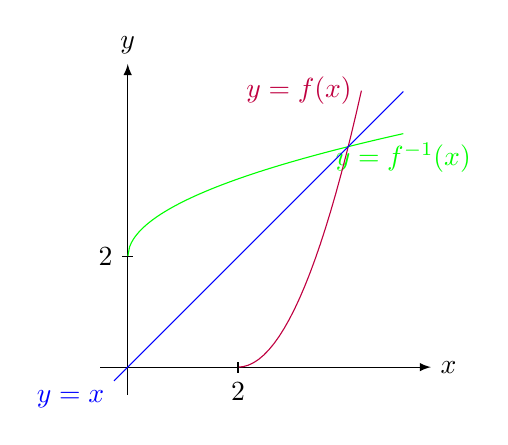
\begin{tikzpicture}[scale=.7]
\draw  [-latex](-0.5,0) -- (5.5,0) node[right]{$x$};
\draw [-latex] (0,-0.5) -- (0,5.5) node[above]{$y$};
\draw [domain=0:5, samples=150, green] plot (\x, {sqrt(\x)+2}) node[below]{$y=f^{-1}(x)$};
\draw [domain=2:4.24, purple] plot (\x, {(\x+-2)^2}) node[left]{$y=f(x)$};
\draw [blue] (-.25,-.25) node[below left]{$y=x$} -- (5,5);
\draw (2,-.1) node [below] {2}--(2,.1);
\draw (-.1,2) node [left] {2}--(.1,2);
\end{tikzpicture}\\
! $Db(f^{-1})$ nur $[2,\infty)$, obwohl $(x-2)^2$ für alle $x \in \mathbb{R}$ erklärt ist.
\end{enumerate}

\paragraph{Def. 6:} \parskp
Die reellwertige Fkt. $y=f(x)$ heißt
\begin{enumerate}[label=\alph*.)]
\item \emph{streng monoton wachsend}, falls $x_1<x_2 \Rightarrow f(x_1)<f(x_2)$ gilt.
\item \emph{monoton wachsend} (=nicht fallend), falls $x_1<x_2 \Rightarrow f(x_1) \leq f(x_2)$ gilt für alle $x_1, x_2 \in Db(f)$.
\item Analog: \emph{Streng monoton fallend} bzw \emph{monoton fallend} (=nicht wachsend).
\end{enumerate}

\paragraph{Satz 2:} \parskp
$f$ streng monoton $\Rightarrow$ $f$ ist injektiv (d.h. $f^{-1}$ existiert)

\subsection{Elementare Funktionen (Teil 2)}

\subsubsection{Wurzel- und Logarithmusfunktionen}
\paragraph{Def. 7:} \parskp
$y=x^{\frac{1}{n}}=\sqrt[n]{x} \qquad (x\in [0,\infty), n \in \mathbb{N}^*)$ ist die Umkehrfunktion zu $y=x^n \quad (x \in [0, \infty))$

\subparagraph{Diskussion: }
\begin{enumerate}
\item Im Bereich der reellen Zahlen ist $\sqrt[n]{x}$ nur für $x\geq 0 $ erklärt, der Funktionswert ist selber nicht negativ.
\item Lässt man in $x^{\frac{1}{3}}$ negative $x$ zu (etwa $\sqrt[3]{-8}=-2$), so ergeben sich Widersprüche:\\
z.B.: $\sqrt[3]{-8}=-2 \Rightarrow -2=-8^{\frac{1}{3}}=(-8)^{\frac{2}{6}}=\left((-8)^2\right)^{\frac{1}{6}}=64^{\frac{1}{6}}=2$
\item Es gilt $\sqrt{x^2}=|x|$ für alle $x \in \mathbb{R}$
\end{enumerate}

\paragraph{Def. 8:}\parskp
$y=log_a (x) \quad (a>0\wedge a \not = 1, x\in (0,\infty))$ ist Umkehrfunktion zu $y=a^x \quad (x \in \mathbb{R})$.\\
Speziell: \begin{itemize}
\item $lg(x):= log_{10}(x)$
\item $ln(x):= log_e (x)$
\end{itemize}
\begin{tikzpicture}[scale=.7]
\draw (1,-.1) node [below] {1}--(1,.1);
\draw (-.1,1) node [left] {1}--(.1,1);
\draw [dashed] (0,1) -- (1,1) -- (1,0);

\draw  [-latex](-3.5,0) -- (5.5,0) node[right]{$x$};
\draw [-latex] (0,-3.5) -- (0,5.5) node[above]{$y$};
\draw [domain=-3:1.6, samples=150] plot (\x, {2.7^\x}) node[right]{$y=a^x$};
\draw [domain=0.05:4, samples=150, green] plot (\x, {ln(\x)}) node[right]{$y=log_a(x)$};

\draw [blue] (-.25,-.25) -- (5,5);
\end{tikzpicture}
\subparagraph{Diskussion:}
\begin{enumerate}
\item Log-Gesetze:
\begin{align*}
log_a(x \cdot y) &= log_a x + log_a y\\
log_a\left(\frac{x}{y}\right) &= log_a x - log_a y\\
log_a(x^{\alpha})&=\alpha \; log_a x\\
log_c b&=\frac{log_a b}{log_a c}
\end{align*}
\item Es gilt $x=a^{log_a x}$ \qquad ($f(f^{-1}(x))=x \forall y \in Db(f^{-1})$)
\item Ferner gilt $a^x=e^{ln(a^x)}=e^{x\cdot ln\;a}$
\end{enumerate}
\subsubsection{Arcusfunktionen}
Vorbetrachtung: $y=f(x)=sin\; x (x \in \mathbb{R})$ ist nicht injektiv, also existiert keine Umkehrfunktion.\\
Aber: $y=\sin(x)$, eingeschränkt auf z.B. $\left[-\frac{\pi}{2}, \frac{\pi}{2}\right]$ ist injektiv und damit umkehrbar.\\
\begin{tikzpicture}[scale=.7]
\draw  [-latex](-6.5,0) -- (6.5,0) node[right]{$x$};
\draw [-latex] (0,-1.5) -- (0,1.5) node[above]{$y$};
\draw [domain= -6:6]plot [smooth] (\x, {sin(\x*66)}) node[right]{$y=\sin(x)$};
\draw [dashed, green] (-1.4,-1.2) node [below] {$-\frac{\pi}{2}$}-- (-1.4,1.2);
\draw [dashed, green] (1.4,-1.2) node [below] {$\frac{\pi}{2}$}-- (1.4,1.2);
\draw [green] (-1.4,0.05) -- (1.4,0.05);
\end{tikzpicture}
\begin{tikzpicture}[scale=1]
\draw  [-latex](-2,0) -- (2,0) node[right]{$x$};
\draw [-latex] (0,-2) -- (0,2) node[above]{$y$};
\begin{scope}[yscale=-1,xscale=1]
\draw [domain= -1.37:1.37, rotate=90]plot [smooth] (\x, {sin(\x*66)}) node [below left]{$y=\arcsin(x)$};
\end{scope}
\draw (-1,-0.1) node [below]{-1} -- (-1,0.1);
\draw (1,-0.1) node [below]{1} -- (1,0.1);
\draw (-0.1,1.37) -- (0.1,1.37) node[right]{$\tfrac{\pi}{2}$};
\draw (-0.1,-1.37) -- (0.1,-1.37) node[right]{$-\tfrac{\pi}{2}$};
\end{tikzpicture}
\paragraph{Def. 9:} \parskp
Umkehrfunktionen\\
\renewcommand{\arraystretch}{1.6}
\begin{tabular}{c | c | c | c l}
 & Db & Wb & Umkehrfunktion von ...\\
\hline
$y=arcsin\; x$ & $[-1,1]$ & $\left[-\frac{\pi}{2}, \frac{\pi}{2}\right]$ & $y=sin\;x$ & $ -\frac{\pi}{2}\leq x \leq \frac{\pi}{2}$\\
$y=arccos\; x $ & $[-1,1]$ & $[0,\pi]$ & $y=cos\; x$ & $0\leq x \leq \pi$\\
$y=arctan\; x$ & $\mathbb{R}$ & $\left(-\frac{\pi}{2}, \frac{\pi}{2}\right)$ & $y=tan \; x $ & $-\frac{\pi}{2}<x<\frac{\pi}{2}$\\
$y=arccot\; x $ & $\mathbb{R}$ & $(0,\pi)$ & $y=cot\; x$ & $0< x <\pi$\\
\end{tabular}
\renewcommand{\arraystretch}{1.3}

\subparagraph{Bsp. 5:}\parskp
Gesucht sind alle Lösungen der folgenden Gleichung: $tan(2x)=y$\\
Es sei $2x \in \left( -\frac{\pi}{2}+k \cdot \pi, \frac{\pi}{2} + k \cdot \pi\right)$, mit $k \in \mathbb{Z}$.\\
$y=tan(2x)=tan(2x-k\cdot \pi)$ mit $2x-k\pi \in \left(-\frac{\pi}{2}, \frac{\pi}{2}\right)$\\
$\Rightarrow 2x - k \pi = arctan(y) \Rightarrow \resultul{x = \frac{arctan(y)+k\pi}{2}}$

\subsubsection{Areafunktionen}

\paragraph{Def. 10:} \parskp
Die Umkehrfunktionen der Hyperbelfunktionen\\
\begin{tabular}{c | c | c | c l}
 & Db & Wb & Umkehrfunktion von ...\\
\hline
$y=\arcsinh\; x$ & $\mathbb{R}$ & $\mathbb{R}$ & $y=\sinh\;x$ & $ x \in \mathbb{R}$\\
$y=\arccosh\; x $ & $[1,\infty)$ & $[0,\infty)$ & $y=cosh\; x$ & $x\geq 0$\\
$y=\arctanh\; x$ & $(-1,1)$ & $\mathbb{R}$ & $y=tanh \; x $ & $x \in \mathbb{R}$\\
$y=\arccoth\; x $ & $\mathbb{R}\setminus[-1,1]$ & $\mathbb{R}\setminus\{0\}$ & $y=coth\; x$ & $x \not = 0$\\
\end{tabular}\\
Aus der Def. der Hyberbelfunktionen (Def. 5) folgt:\\
$\arcsinh\; x = ln (x+\sqrt{x^2+1})$\\
$\arctanh\; x=\frac{1}{2}ln\left(\frac{1+x}{1-x}\right)$\\
$\arccosh\; x = ln (x+\sqrt{x^2+1}$\\
$\arccoth\; x = \frac{1}{2}ln\left(\frac{x+1}{x-1}\right)$